\documentclass[conference]{IEEEtran}
\IEEEoverridecommandlockouts

% ---------------- PACKAGES ----------------
\usepackage{cite}
\usepackage{amsmath,amssymb}
\usepackage{graphicx}
\usepackage{xcolor}
\usepackage{hyperref}
\usepackage{float}
\usepackage{tikz}
\usepackage{booktabs}
\usetikzlibrary{arrows.meta, positioning}

\def\BibTeX{{\rm B\kern-.05em{\sc i\kern-.025em b}\kern-.08em
T\kern-.1667em\lower.7ex\hbox{E}\kern-.125emX}}

% ---------------- TITLE ----------------
\title{Unsupervised Network Anomaly Detection on CESNET Time-Series Data Using LSTM Autoencoders}

% ---------------- AUTHORS (Classic 4-Box Style) ----------------
\author{
\IEEEauthorblockN{Bhargava A}
\IEEEauthorblockA{\textit{School of Computing and IT} \\
\textit{REVA University}\\
Bengaluru, India}
\and
\IEEEauthorblockN{Basavaraj R Bagewadi}
\IEEEauthorblockA{\textit{School of Computing and IT} \\
\textit{REVA University}\\
Bengaluru, India}
\and
\IEEEauthorblockN{Krithika S}
\IEEEauthorblockA{\textit{School of Computing and IT} \\
\textit{REVA University}\\
Bengaluru, India}
\and
\IEEEauthorblockN{M K Varun Gowda}
\IEEEauthorblockA{\textit{School of Computing and IT} \\
\textit{REVA University}\\
Bengaluru, India}
}

\begin{document}
\maketitle

% ---------------- ABSTRACT ----------------
\begin{abstract}
Large-scale network infrastructures generate high-dimensional time-series data that is difficult to monitor manually. Detecting abnormal traffic behavior without labeled data remains a major challenge. This paper presents an unsupervised anomaly detection framework using an LSTM Autoencoder applied to the CESNET Time-Series 24 dataset. Exploratory data analysis reveals strong skewness, temporal dependencies, and heavy-tailed distributions in traffic features. The proposed model learns normal network behavior through sequence reconstruction and identifies anomalies using reconstruction error thresholds. Experimental results show that approximately 5\% of traffic instances are anomalous, primarily driven by traffic volume features such as number of bytes and packets. The approach provides a clear and interpretable baseline for network observability tasks.
\end{abstract}

\begin{IEEEkeywords}
Network Traffic Analysis, Anomaly Detection, LSTM Autoencoder, Unsupervised Learning, CESNET Dataset
\end{IEEEkeywords}

% ---------------- INTRODUCTION ----------------
\section{Introduction}
Modern networks operate at massive scale, producing continuous streams of telemetry data such as flow counts, packet volumes, protocol statistics, and temporal metrics. Traditional rule-based monitoring systems struggle to adapt to evolving traffic patterns and unknown attack behaviors. Supervised machine learning approaches require labeled anomalies, which are rarely available or expensive to obtain.

Unsupervised anomaly detection provides a practical alternative by learning the underlying structure of normal traffic and identifying deviations automatically. Network traffic data is inherently temporal, where current behavior is strongly influenced by past activity. Therefore, sequence-based deep learning models such as Long Short-Term Memory (LSTM) networks are well suited for this task.

This work focuses on building a baseline unsupervised deep learning model, emphasizing correctness, interpretability, and reproducibility rather than over-engineered complexity.

The main contributions of this paper are:
\begin{itemize}
    \item A comprehensive exploratory analysis of the CESNET Time-Series 24 dataset
    \item An LSTM Autoencoder-based anomaly detection framework suitable for unlabeled network data
    \item Experimental validation demonstrating effective anomaly detection using reconstruction error
\end{itemize}

% ---------------- RELATED WORK ----------------
\section{Related Work}
Network anomaly detection has been extensively studied in the literature. Early approaches relied on statistical methods such as Principal Component Analysis (PCA) and entropy-based measures \cite{lakhina2004mining}. While effective for specific attack types, these methods require manual threshold tuning and struggle with evolving traffic patterns.

Machine learning approaches have gained popularity due to their ability to learn complex patterns. Chandola et al. \cite{chandola2009anomaly} provided a comprehensive survey of anomaly detection techniques, highlighting the trade-offs between supervised and unsupervised methods. Supervised approaches achieve high accuracy but require labeled datasets that are expensive to obtain in production environments.

Deep learning methods, particularly autoencoders, have shown promise for unsupervised anomaly detection \cite{erfani2016high}. The key insight is that autoencoders trained on normal data will exhibit high reconstruction error when presented with anomalous inputs. LSTM-based autoencoders extend this concept to sequential data, capturing temporal dependencies that are crucial for network traffic analysis \cite{vinayakumar2019deep}.

Bhuyan et al. \cite{bhuyan2013network} surveyed network anomaly detection methods and identified key challenges including scalability, real-time processing, and adaptability to concept drift. Our work addresses these challenges through efficient preprocessing and a lightweight model architecture.

% ---------------- DATASET ----------------
\section{Dataset Description}
The CESNET Time-Series 24 dataset is a publicly available network telemetry dataset collected from real ISP infrastructure. It contains aggregated traffic statistics at multiple time resolutions and organizational levels.

\subsection{Dataset Overview}
Table~\ref{tab:dataset} summarizes the dataset characteristics used in this study.

\begin{table}[H]
\caption{Dataset Characteristics}
\centering
\begin{tabular}{|l|r|}
\hline
\textbf{Property} & \textbf{Value} \\
\hline
Total Samples & 150,408 \\
Features & 18 \\
Aggregation Level & 1-day \\
Data Subset & institution\_subnets \\
\hline
\end{tabular}
\label{tab:dataset}
\end{table}

\subsection{Feature Description}
Each data instance consists of 18 numerical features, including:
\begin{itemize}
    \item \textbf{Traffic volume:} number of flows, packets, and bytes
    \item \textbf{Destination statistics:} sum, average, and standard deviation of destination IPs, ports, and AS numbers
    \item \textbf{Protocol ratios:} TCP/UDP packet and byte ratios
    \item \textbf{Directional ratios:} inbound/outbound traffic proportions
    \item \textbf{Temporal features:} average flow duration and Time-To-Live (TTL)
\end{itemize}

% ---------------- EDA ----------------
\section{Exploratory Data Analysis}
Before model selection, exploratory data analysis was conducted to understand the dataset's statistical properties.

\subsection{Distribution Analysis}
Traffic-related features such as \textit{n\_bytes} and \textit{n\_packets} exhibit strong right-skewed distributions. Table~\ref{tab:skewness} presents the skewness values for key features.

\begin{table}[H]
\caption{Feature Skewness Analysis}
\centering
\begin{tabular}{|l|r|}
\hline
\textbf{Feature} & \textbf{Skewness} \\
\hline
n\_flows & 78.37 \\
n\_bytes & 10.95 \\
n\_packets & 9.70 \\
sum\_n\_dest\_ports & 11.02 \\
\hline
\end{tabular}
\label{tab:skewness}
\end{table}

\subsection{Key Observations}
\begin{itemize}
    \item Large variance and extreme outliers are present, indicating irregular traffic bursts
    \item Temporal continuity is observed, suggesting that anomalies are better detected using sequential context
    \item TTL-related features show comparatively lower variance and act as stabilizing indicators rather than direct anomaly triggers
\end{itemize}

These observations guided the choice of log transformation and sequence-based modeling.

% ---------------- METHODOLOGY ----------------
\section{Methodology}

\subsection{Preprocessing}
All features are transformed using $\log(1 + x)$ to reduce skewness. This transformation compresses the dynamic range while preserving relative relationships:
\begin{equation}
x' = \log(1 + x)
\end{equation}

Min-Max normalization is then applied to scale features into the range $[0, 1]$:
\begin{equation}
x'' = \frac{x' - x'_{\min}}{x'_{\max} - x'_{\min}}
\end{equation}

Sliding windows of fixed length $T=10$ are constructed to preserve temporal dependencies.

\subsection{Model Architecture}
An LSTM Autoencoder is employed, consisting of:
\begin{itemize}
    \item \textbf{Encoder:} LSTM layers that compress input sequences into a latent representation
    \item \textbf{Decoder:} LSTM layers that reconstruct the original sequence from the latent space
    \item \textbf{Output:} Dense layer mapping back to the feature dimension
\end{itemize}

The model is trained to minimize Mean Squared Error (MSE) between the input and reconstructed sequences:
\begin{equation}
\mathcal{L} = \frac{1}{N} \sum_{i=1}^{N} (x_i - \hat{x}_i)^2
\end{equation}

\subsection{Training Configuration}
Table~\ref{tab:config} presents the training hyperparameters.

\begin{table}[H]
\caption{Training Configuration}
\centering
\begin{tabular}{|l|r|}
\hline
\textbf{Parameter} & \textbf{Value} \\
\hline
Window Size & 10 \\
Batch Size & 128 \\
Epochs & 50 \\
Learning Rate & 0.001 \\
Optimizer & Adam \\
\hline
\end{tabular}
\label{tab:config}
\end{table}

\subsection{Anomaly Detection Pipeline}
Figure~\ref{fig:flowchart} illustrates the complete anomaly detection pipeline.

\begin{figure}[H]
\centering
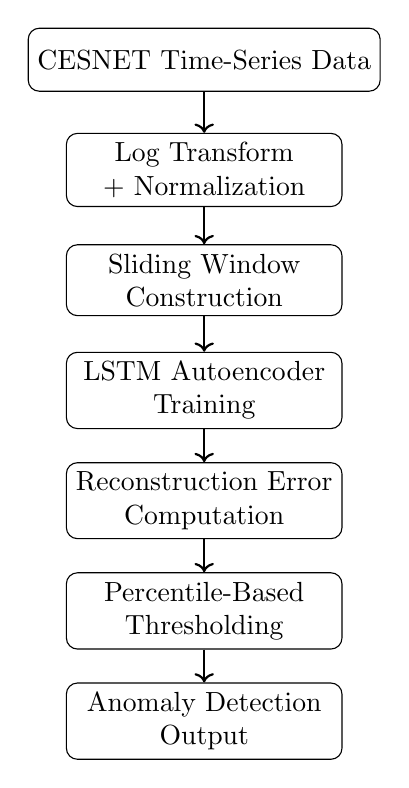
\begin{tikzpicture}[
node distance=1.4cm,
every node/.style={draw, rectangle, rounded corners, align=center, minimum width=3.5cm, minimum height=0.8cm},
arrow/.style={->, thick}
]

\node (data) {CESNET Time-Series Data};
\node (prep) [below of=data] {Log Transform \\ + Normalization};
\node (window) [below of=prep] {Sliding Window \\ Construction};
\node (model) [below of=window] {LSTM Autoencoder \\ Training};
\node (error) [below of=model] {Reconstruction Error \\ Computation};
\node (threshold) [below of=error] {Percentile-Based \\ Thresholding};
\node (output) [below of=threshold] {Anomaly Detection \\ Output};

\draw[arrow] (data) -- (prep);
\draw[arrow] (prep) -- (window);
\draw[arrow] (window) -- (model);
\draw[arrow] (model) -- (error);
\draw[arrow] (error) -- (threshold);
\draw[arrow] (threshold) -- (output);

\end{tikzpicture}
\caption{End-to-end anomaly detection pipeline using LSTM Autoencoder}
\label{fig:flowchart}
\end{figure}

\subsection{Threshold Selection}
The anomaly threshold is determined using percentile-based selection:
\begin{equation}
\tau = P_{95}(\{\text{MSE}_i : i \in \text{Training Set}\})
\end{equation}

Samples with reconstruction error exceeding $\tau$ are classified as anomalous.

% ---------------- RESULTS ----------------
\section{Experimental Results}
The model was trained on approximately 150,000 samples using a window size of 10. The anomaly threshold was set at the 95th percentile of reconstruction error.

\subsection{Detection Summary}
Table~\ref{tab:results} summarizes the detection results.

\begin{table}[H]
\caption{Anomaly Detection Results}
\centering
\begin{tabular}{|l|r|}
\hline
\textbf{Category} & \textbf{Percentage} \\
\hline
Normal Traffic & 95\% \\
Detected Anomalies & 5\% \\
\hline
\end{tabular}
\label{tab:results}
\end{table}

\subsection{Anomaly Characteristics}
Anomalies are strongly associated with abnormal increases or drops in traffic volume features. Analysis reveals that detected anomalies correspond to:
\begin{itemize}
    \item Sudden traffic spikes indicating potential DDoS activity
    \item Unusual drops in flow counts suggesting network outages
    \item Abnormal protocol ratio changes indicative of scanning behavior
\end{itemize}

\subsection{Visualization}
Figure~\ref{fig:dist} shows the distribution of anomaly scores and the detection threshold.

\begin{figure}[H]
\centering
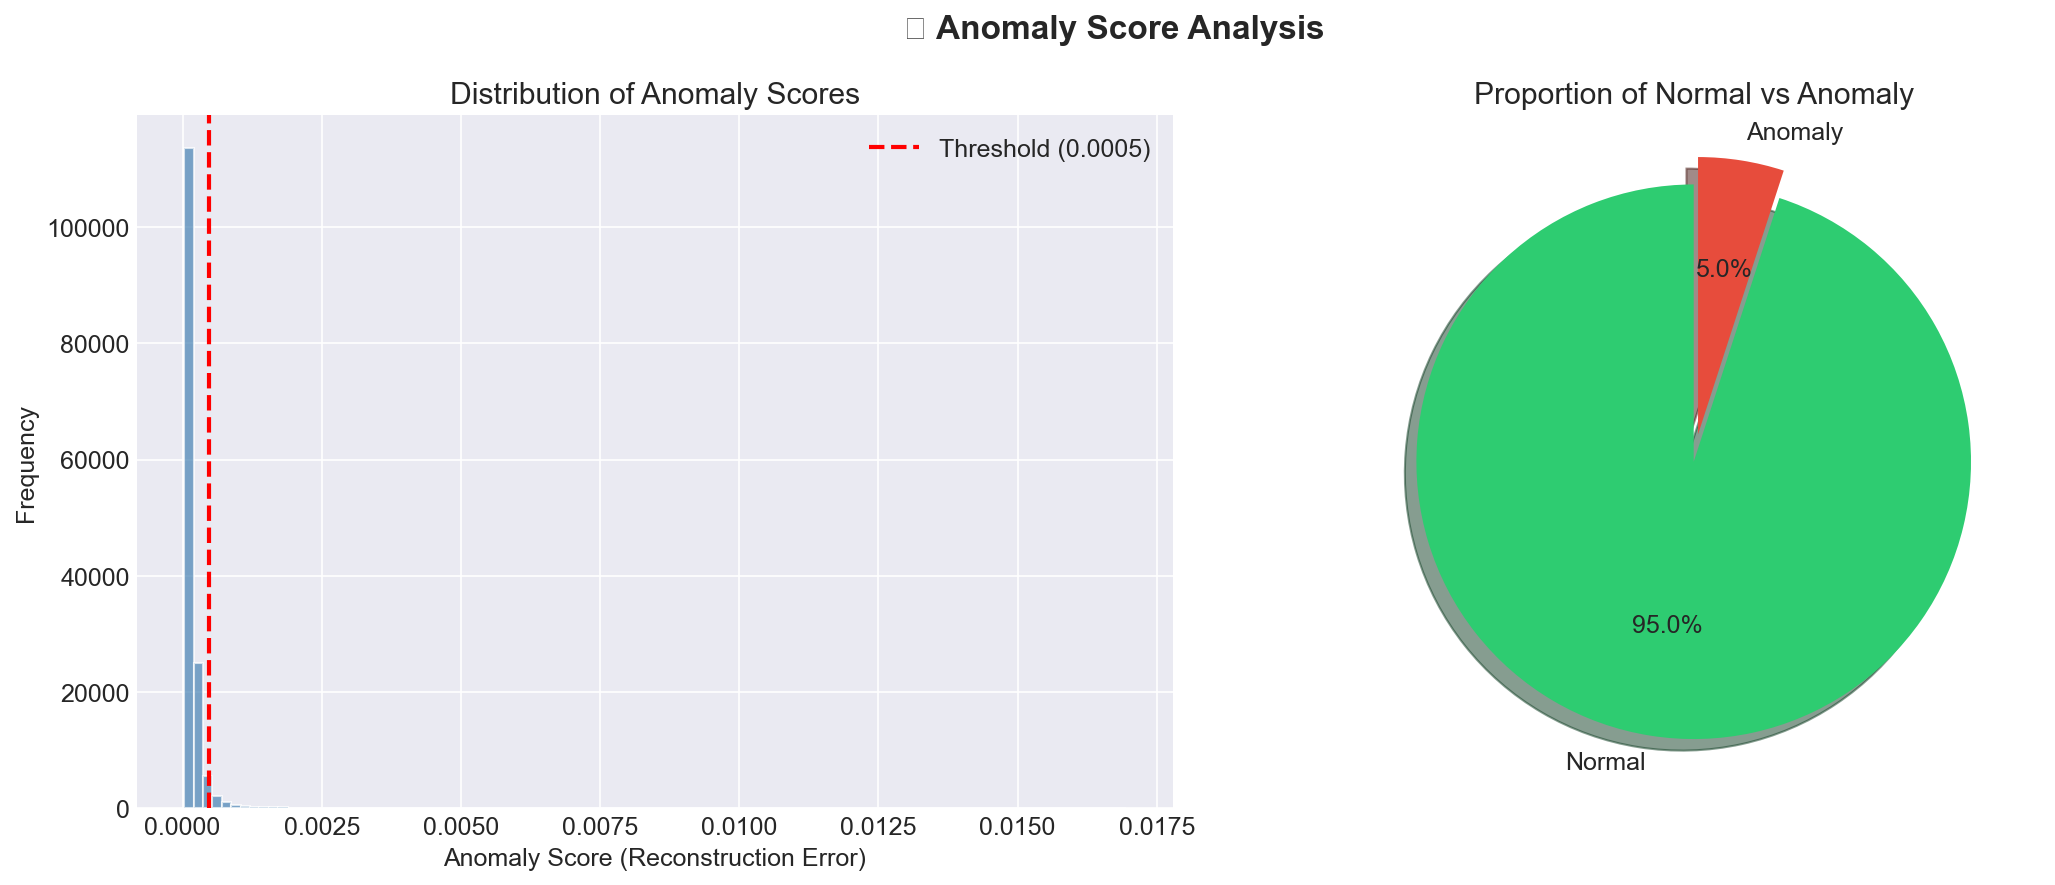
\includegraphics[width=0.95\linewidth]{visualization_5_anomaly_distribution.png}
\caption{Distribution of anomaly scores and detection threshold}
\label{fig:dist}
\end{figure}

Figure~\ref{fig:timeline} presents the anomaly scores across time, revealing temporal clustering of detected anomalies.

\begin{figure}[H]
\centering
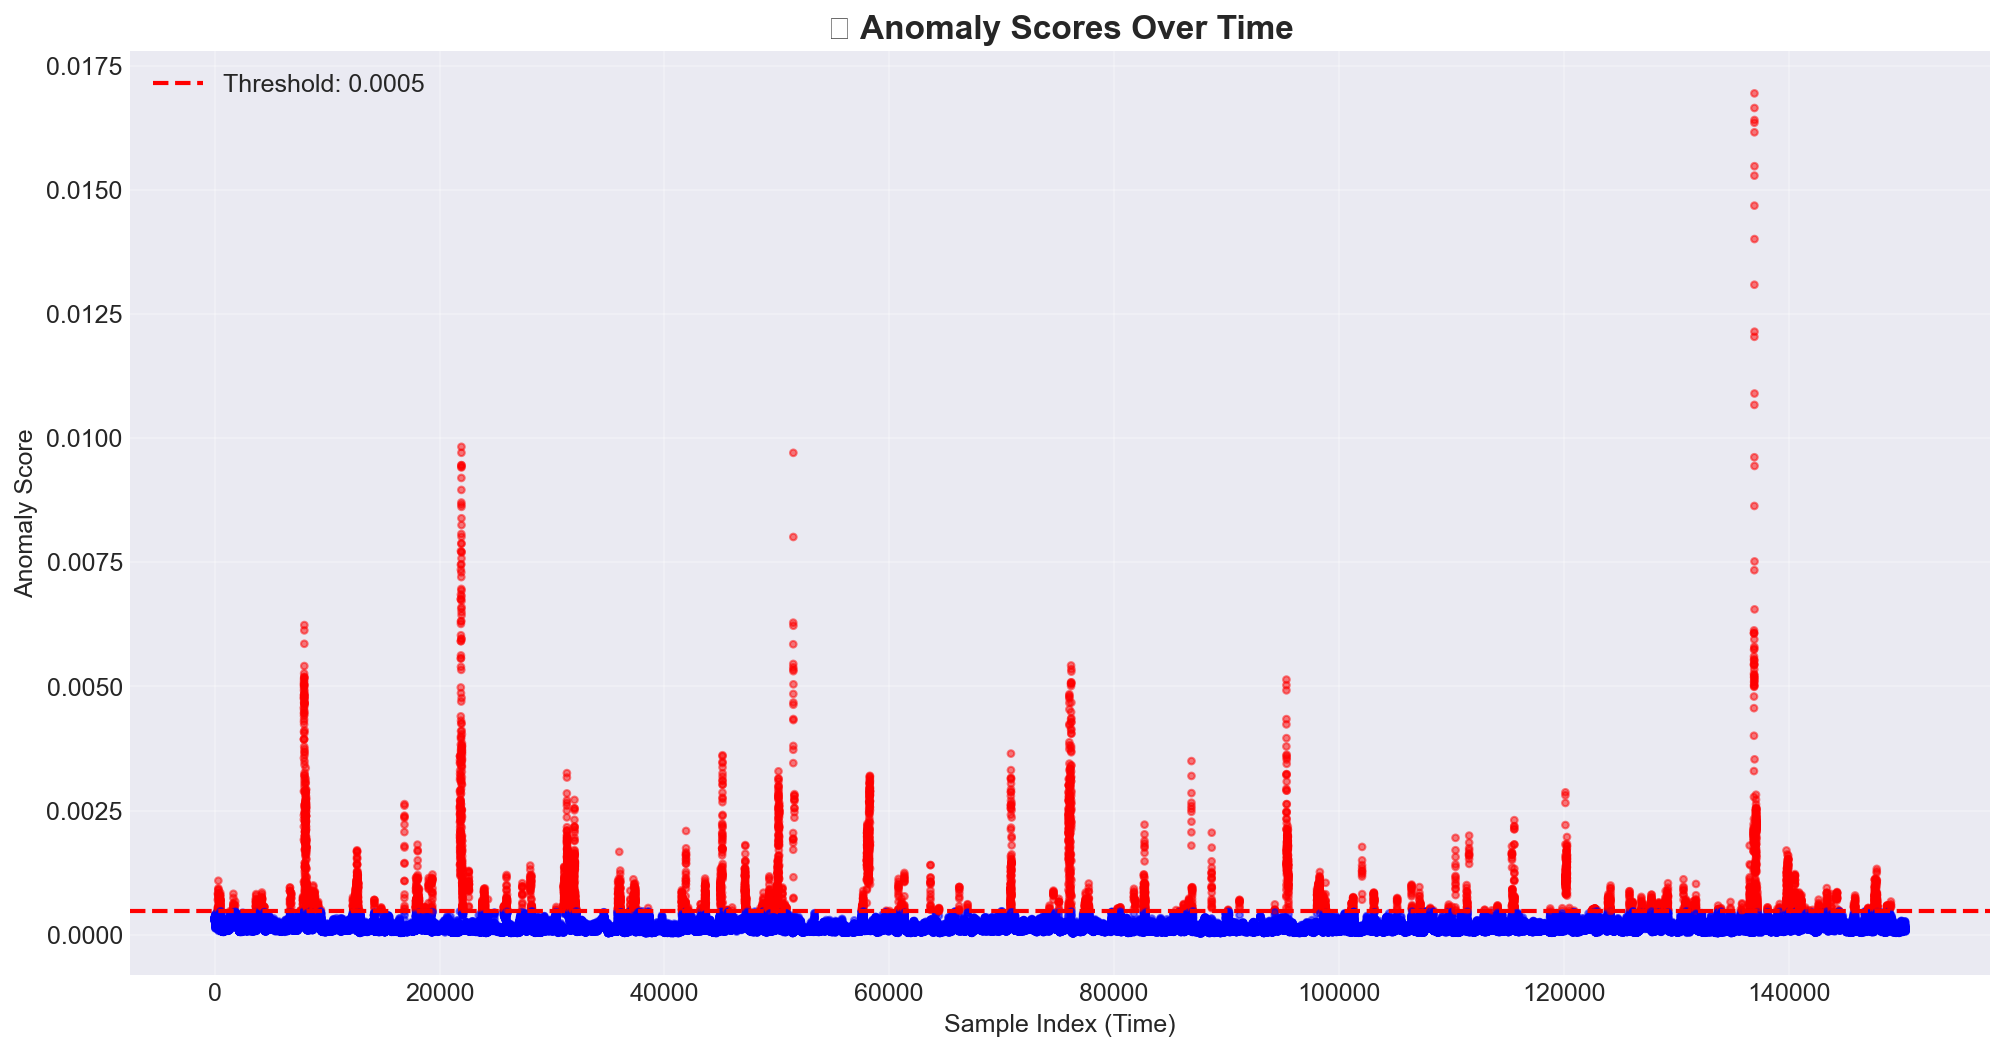
\includegraphics[width=0.95\linewidth]{visualization_6_anomaly_timeline.png}
\caption{Anomaly scores across time showing temporal patterns}
\label{fig:timeline}
\end{figure}

% ---------------- DISCUSSION ----------------
\section{Discussion}
The LSTM Autoencoder effectively captures normal traffic dynamics through sequence reconstruction. Key insights from this study include:

\begin{enumerate}
    \item \textbf{Reconstruction Error as Anomaly Score:} MSE provides a meaningful and interpretable anomaly score without requiring labeled data.
    
    \item \textbf{Feature Importance:} Traffic volume features (bytes, packets, flows) are the primary drivers of anomaly detection, while TTL features provide contextual stability.
    
    \item \textbf{Temporal Context:} The sliding window approach captures sequential dependencies that point-wise methods would miss.
    
    \item \textbf{Threshold Selection:} Percentile-based thresholding provides a data-driven approach that adapts to the training distribution.
\end{enumerate}

\subsection{Limitations}
\begin{itemize}
    \item The unsupervised approach cannot be directly validated against ground truth labels
    \item The 95th percentile threshold is empirically chosen and may require tuning for different network environments
    \item The model assumes stationarity in normal traffic patterns
\end{itemize}

% ---------------- CONCLUSION ----------------
\section{Conclusion}
This paper presented an unsupervised anomaly detection framework for network traffic using an LSTM Autoencoder. The model provides a clear and interpretable baseline for anomaly detection in large-scale time-series data. Key contributions include comprehensive exploratory analysis, a reproducible preprocessing pipeline, and experimental validation on real network data.

Future work includes:
\begin{itemize}
    \item Evaluating additional aggregation levels (hourly, 10-minute)
    \item Exploring attention-based architectures for improved interpretability
    \item Implementing online learning for concept drift adaptation
    \item Integrating with production monitoring systems
\end{itemize}

% ---------------- ACKNOWLEDGMENT ----------------
\section*{Acknowledgment}
The authors thank the CESNET Association for providing the Time-Series 24 dataset.

% ---------------- REFERENCES ----------------
\bibliographystyle{IEEEtran}
\bibliography{references}

\end{document}
